\apendice{Especificación de diseño}

\section{Introducción}
En esta parte del anexo definiremos como se han resuelto los objetivos expuestos anteriormente.
\section{Diseño de datos}
El proyecto cuenta con las siguientes entidades:
\begin{itemize}
	\item \textbf{Homogeneous Ensemble}: Es la superclase de los distintos algoritmos que hemos realizado, todos tienen unos parámetros en común. Por defecto, nos hace un \texttt{ExtraTreeClassifier}.
	\item \textbf{Disturbing Neighbors}: El método crea características nuevas que se agregarán al conjunto de datos del clasificador base. Dichas características se calculan con el clasificador Nearest Neighbour(NN), construido a partir de unas instancias seleccionadas al azar. Para probar la eficacia utilizamos árboles de decisión como clasificador base. 
	\item \textbf{Random Oracles}: Cada clasificador del conjunto se reemplaza por un miniensemble de un par de subclasificadores con un oráculo para elegir entre ellos.
	\item \textbf{Rotation Forest}: Este método genera conjuntos de clasificadores basados en la extracción de características. Crea un conjunto de entrenamiento para un clasificador base, este conjunto se divide al azar en subconjunto. La idea es mejorar la precisión y diversidad dentro del conjunto. La diversidad se basa en la extracción de características para cada clasificador base.
\end{itemize}


\subsection{Diagrama de clases general}\label{diagram-general}
En esta parte vamos hacer una breve explicación de la función que tiene cada clase.
\begin{itemize}
	\item \textbf{BaseEstimator}: Es la que utilizan todos los clasificadores de Scikit-Learn.
	\item \textbf{BaseEnsemble}: Hereda de \textbf{BaseEstimator}.Es la clase que utilizan todos los ensembles.
	\item \textbf{ClassifierMixin}: Es la clase para todos los clasificadores de Scikit-Learn, ya que esta tiene el método \textit{score}.
	\item \textbf{HomogeneousEnsemble}: Hereda de \textbf{BaseEnsemble}. Es una superclase, que es la que utilizan los \textit{ensembles}  que hemos realizado, ya que todos tienen unos parámetros en común.
	\item \textbf{DisturbingNeighbors}: Hereda de \textbf{HomogeneousEnsemble}. Esta clase es un ensemble que usa el clasificador \textbf{BaseDisturbingNeighbors}, para realizar las predicciones de los conjuntos de datos.
	\item \textbf{RandomOracles}: Hereda de \textbf{HomogeneousEnsemble}. Esta clase es un ensemble que usa el clasificador \textbf{BaseRandomOracles}, para realizar las predicciones de los conjuntos de datos.
	\item \textbf{RotationForest}: Hereda de \textbf{HomogeneousEnsemble}. Esta clase es un ensemble que usa el clasificador \textbf{BaseRotationForest}, para realizar las predicciones de los conjuntos de datos.
	\item \textbf{BaseDisturbingNeighbors}: Hereda de \textbf{ClassifierMixin} y de \textbf{BaseEstimator}, y es una agregación de \textbf{DisturbingNeighbors}. Es un clasificador base.
	\item \textbf{BaseRandomOracles}: Hereda de \textbf{ClassifierMixin}, y es una agregación de \textbf{RandomOracles}. Es un clasificador base.
	\item \textbf{BaseRotationForest}: Hereda de \textbf{ClassifierMixin} y de \textbf{BaseEstimator}, y es una agregación de \textbf{RotationForest}. Es un clasificador base.
\end{itemize}
Podemos ver un esquema de como son las relaciones en~\ref{fig:DiagramGeneral}

\begin{figure}
\centering
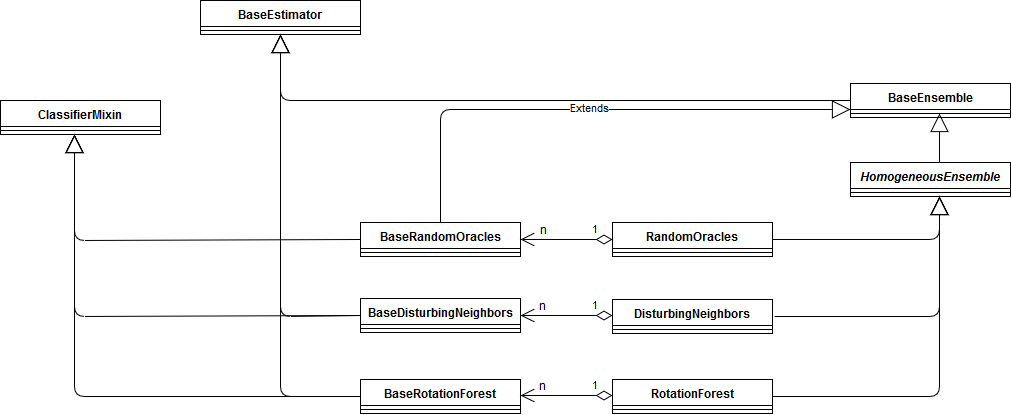
\includegraphics[width=0.95\textwidth]{DiagramGeneral}
\caption{Diagrama de clases general}
\label{fig:DiagramGeneral}
\end{figure}

\subsection{Diagrama de clases implementadas}\label{diagram-implement}
En este diagrama podremos apreciar cada una de las clases implementadas, y sus parámetros y métodos~\ref{fig:DiagramImplement}.
\begin{itemize}	
	\item \textbf{HomogeneousEnsemble}: Los parámetros que contiene esta clase son base\_estimator, que por defecto tiene \textbf{ExtraTreeClassifier}, otro sería el nº de estimadores, que son las iteraciones que haremos sobre nuestro clasificador base. Tiene tres métodos \textit{fit}, \textit{predict} y  \textit{predict\_proba}, en donde se calcula el promedio de los clasificadores base.
	\item Los tres ensembles \textbf{DisturbingNeighbors}, \textbf{RandomOracles} y \textbf{RotationForest}, tienen los parámetros que son específicos de cada clasificador base.
	\item Los clasificadores base \textbf{BaseDisturbingNeighbors}, \textbf{BaseRandomOracles} y \textbf{BaseRotationForest}, cada uno tiene sus parámetros específicos, y cada uno tiene los métodos necesarios para predecir el conjunto de datos.
\end{itemize}

\begin{figure}
\centering
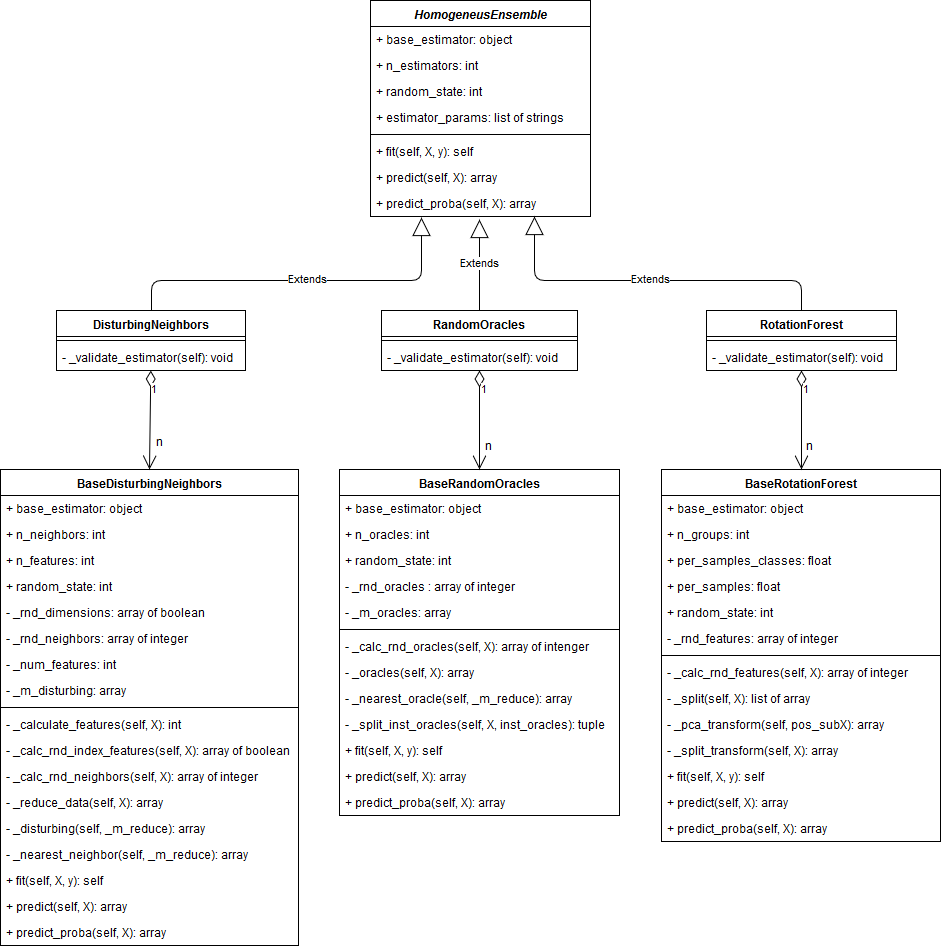
\includegraphics[width=0.95\textwidth]{DiagramImplement}
\caption{Diagrama de clases implementadas}
\label{fig:DiagramImplement}
\end{figure}

\section{Diseño procedimental}
\subsection{Diagrama de secuencias}\label{diagrama-secuencias}
Se ha realizado un diagrama de secuencias de como seria un ejemplo de ejecución del \textit{ensemble} Disturbing Neighbors, que podemos ver en~\ref{fig:DiagramSequence}.

Los pasos que se han llevado son:
\begin{itemize}
	\item Creamos el clasificador \texttt{DistubingNeighbors} que a su vez este creara el clasificador base \texttt{BaseDisturbingNeighbors}, y este a su vez \texttt{DecicisionTreeClassifier}.
	\item Una vez creado el clasificador, tendremos tantos clasificadores base como iteraciones tenga nuestro \textit{ensemble}  DisturbingNeighbors. Cada uno de estos clasificadores base entrara el conjunto de datos que le pasamos.
	\item Una vez tengamos nuestros clasificadores base entrenados, lo próximo es hacer la predicción de cada uno de ellos. Que igual que en el entrenamiento se hace sobre cada uno de los clasificadores. Pero lo que al final devolvemos es el promedio de todas las predicciones de los clasificadores base.
	\item Por último realizamos las predicciones de probabilidad, que estas lo que nos devolverán será la probabilidad de cada una de las clases de que sean 1 o 0. Al igual que en las predicciones, se calcula el promedio de todas. Aunque en la imagen no este no está reflejado, ya que básicamente sería igual que las predicciones. 
\end{itemize}
\begin{figure}
\centering
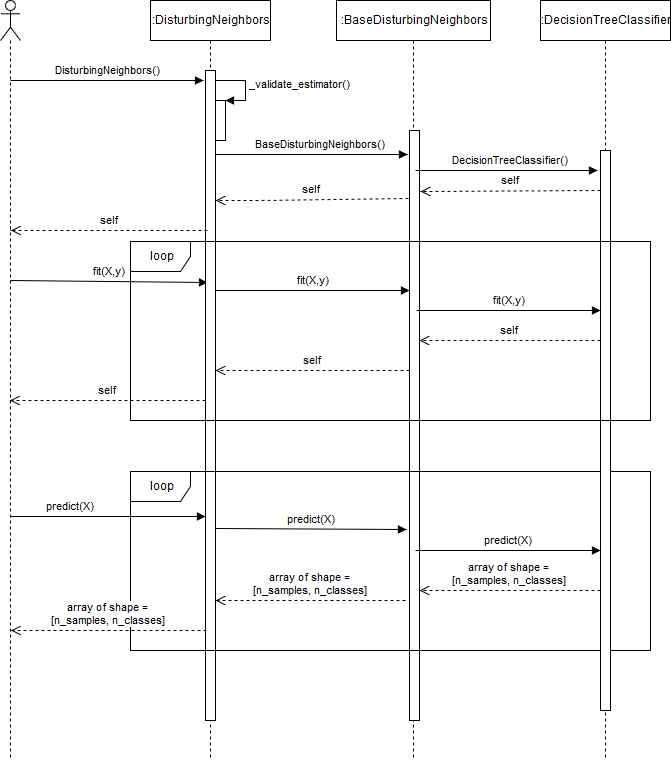
\includegraphics[width=0.95\textwidth]{DiagramSequence}
\caption{Diagrama de secuencias del funcionamiento de un Notebook}
\label{fig:DiagramSequence}
\end{figure}

\section{Diseño arquitectónico}
En esta sección, vamos a explicar y mostrar de forma general como esta diseñado el proyecto y como es la distribución de paquetes, que podemos ver en~\ref{fig:DiagramArchitectural}.

Vamos hacer una descripción sobre cada paquete y su contenido.
\begin{itemize}
	\item Sklearn-ubu: Este paquete contendrá todos los ficheros del código fuente de nuestro proyecto, es decir, los clasificadores base y los \textit{ensembles}.
	
	\item Sklearn: Aunque este paquete no pertenece a este proyecto, como los algoritmos que hemos realizado, queremos implementarlos en la librería de Scikit-Learn, ha sido necesario hacer usos de este paquete en algunas ocasiones, por ello lo incluimos.
	
\end{itemize}
\begin{figure}
\centering
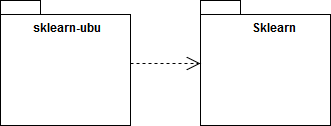
\includegraphics[width=0.50\textwidth]{DiagramArchitectural}
\caption{Diagrama de la estructura}
\label{fig:DiagramArchitectural}
\end{figure}
